\section{Backlog}
% JT Week 2
% complete

% Figure here
\subsubsection{Prototype 1}
\begin{figure}[H]
    \centering
    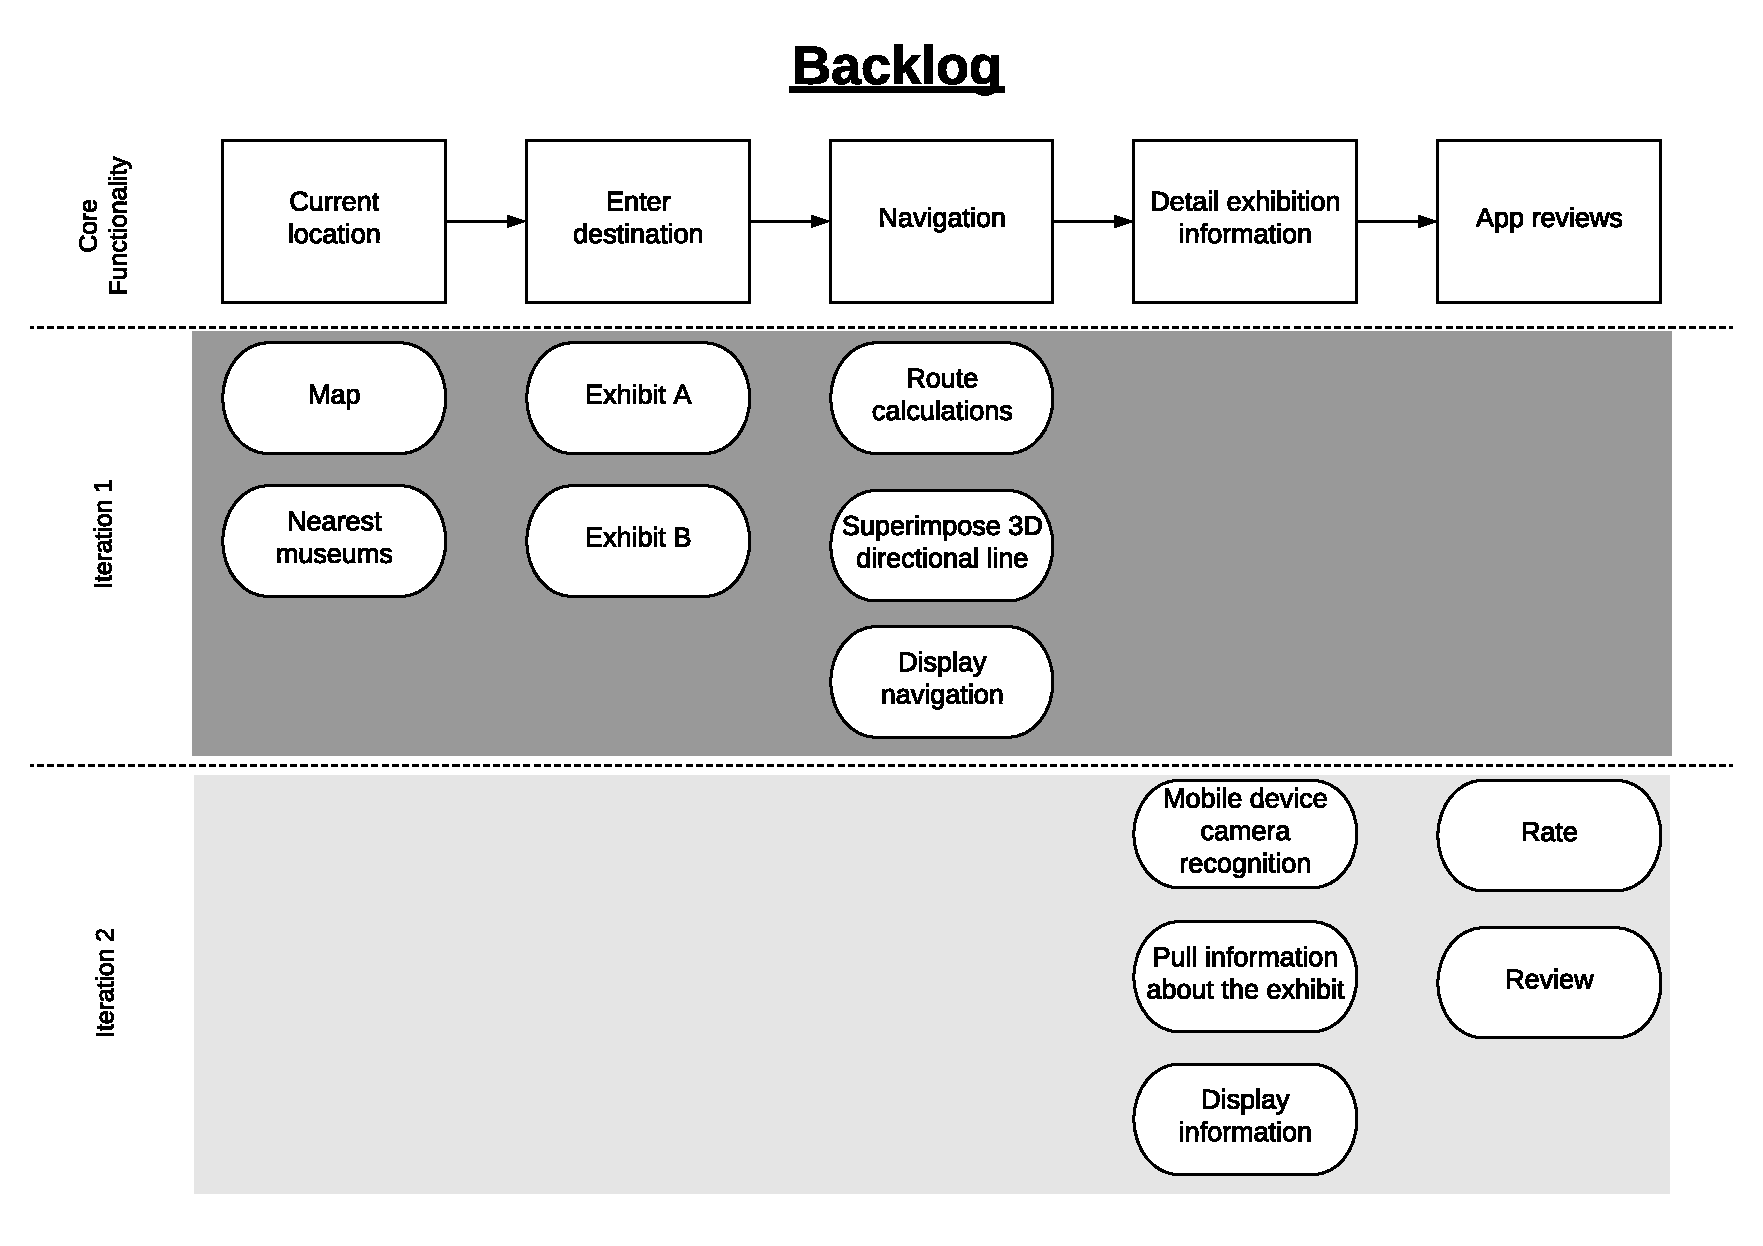
\includegraphics[width=\textwidth]
    {technicalarchitecture/backlog.pdf}
    \caption{Inital Product Backlog}
    \label{fig:productbacklog}
\end{figure}

The product backlog was used as the single source of requirements in order to prioritise releases and allow for transparent iteration planning. From the requirements, and project scope each of the five core functionalities were broken down into its major components. Considering the time estimates, the scrum team decided that to demonstrate originality in the project, and to build the base functionalities first, both the route calculations and the AR implementation were to form the MVP. Features which required a database such as exhibition item/image recognition, and user profiles/logins were placed in the app's second release. These components would take longer than the amount of development time available along with the base functionalities. The team recognised the added time for the construction and integration of a database to the app would increase the risk in not delivering a functional MVP. As a living scrum artifact, the backlog changed accordingly when there were requirements, enhancements and fixes during the implementation and testing phases of each sprint.

% table of time estimates
\begingroup
\renewcommand{\arraystretch}{1.5} % Default value: 1
\begin{table}[H]
\centering
\begin{tabular}{l|c}
% \begin{tabular}{| >{\centering\arraybackslash} | >{\centering\arraybackslash} |}
\textbf{Function}                & \textbf{Estimate Time (Days)} \\ \hline
Displaying map                   & 0.5                           \\
Finding nearest museums          & 3                             \\
Getting start and end locations  & 5                             \\
Route calculations               & 10                            \\
Superimpose 3D directional line  & 12                            \\
Displaying navigation            & 10                            \\
Mobile device camera recognition & 2                             \\
Retrieve exhibit information     & 10                            \\
Display exhibit information      & 1                             \\
Rating the app                   & 1                             \\
Reviewing the museum visit       & 3                             
\end{tabular}
\caption{Table of time estimates for each function}
\label{table:timeestimates}
\end{table}
\endgroup

\section{Sprint Outlines}
% JT Week 2
% complete
During implementation, four sprints were conducted each lasting one to two weeks. The first sprint lasting one week with the goal of building a beacon for calculating distances between users and objects. The follow sprint focused on route calculations; being able to calculate the route between two points in a given space. For the AR part, this was divided into two separate sprint, with the initial one focusing on rendering and anchoring objects in real-time, and afterwards the integration with all base functionalities.

\section{Front-end}
% Hamza Week 2

Front-end development was carried out in Java on Android Studio. 

It was carried out in the early stages of implementation due to the fact that the team had already recieved user feedback for the UI/UX prototypes. After combining the positive features of the initial design prototypes into one, it became easier to visualise the end-result. With aims to create an user interface that is user friendly and intuitive, various features of the application are self-explanatory. 

As soon as the application is opened, the user is faced with the login page asking for credentials. The idea behind having a user account system is so that the user can keep track of their past visits to museums and review various sites; this was an idea that was put in place for future developments but was not included in the MVP. However, if the user does not have an account they are also able to 'Continue as a Guest' and use the services freely without saving any data. The forms are easy to fill in that does involve any technical complexity.

When the user has passed the login page, they are able to see the menu. The menu has three different services that the user can utilise. The first being the 'Map' which shows the user their current location and their surroundings on a 2D map. The 'Nav' menu takes the user to the screen which the user has to then enter their desired destination or exhibit. After all the information has been entered by the user, the user's device displays the AR-enabled camera with the highlighted navigational line directing the user to their destination. However, if the user's device is not compatible with Google's ARCore SDK then the user will not be able to see this screen and are instead faced with an error message. Lastly, the 'info' page will allow the user to see additional information about a specific exhibit of their choice - this also requires the user to fill out a simple form.

As a result of all the planning and prototyping, when it came to actualising the design in Android Studio it was as simple as writing code for implementation - no further designing was needed, with exception of minor changes such as font sizes.

\note{can we add some screenshots?}

\section{Back-end}
% Gabe Week 2
% still needs work
% complete after integration

\note{You can still talk about loads of things, just not the integration bit}

\section{Hardware}
% Nick Week 2
% complete
It was devised that the project needed to pursue a hardware solution which would be able to transmit the user’s location to compute a route solution. Utilising the Arduino (UNO R3 Mega 2560)’s small foot-print, a simple beacon plan was sought consisting of the Arduino coupled with the Bluetooth HC- 05 RF transceiver. 
 
Figure~\ref{fig:arduino} displays the basic layout of the beacon aside from power input via the board’s USB-B socket. This configuration was able to send the strength of the Bluetooth frequency thereby allowing the computation of a distance.

% figure here
\begin{figure}[H]
    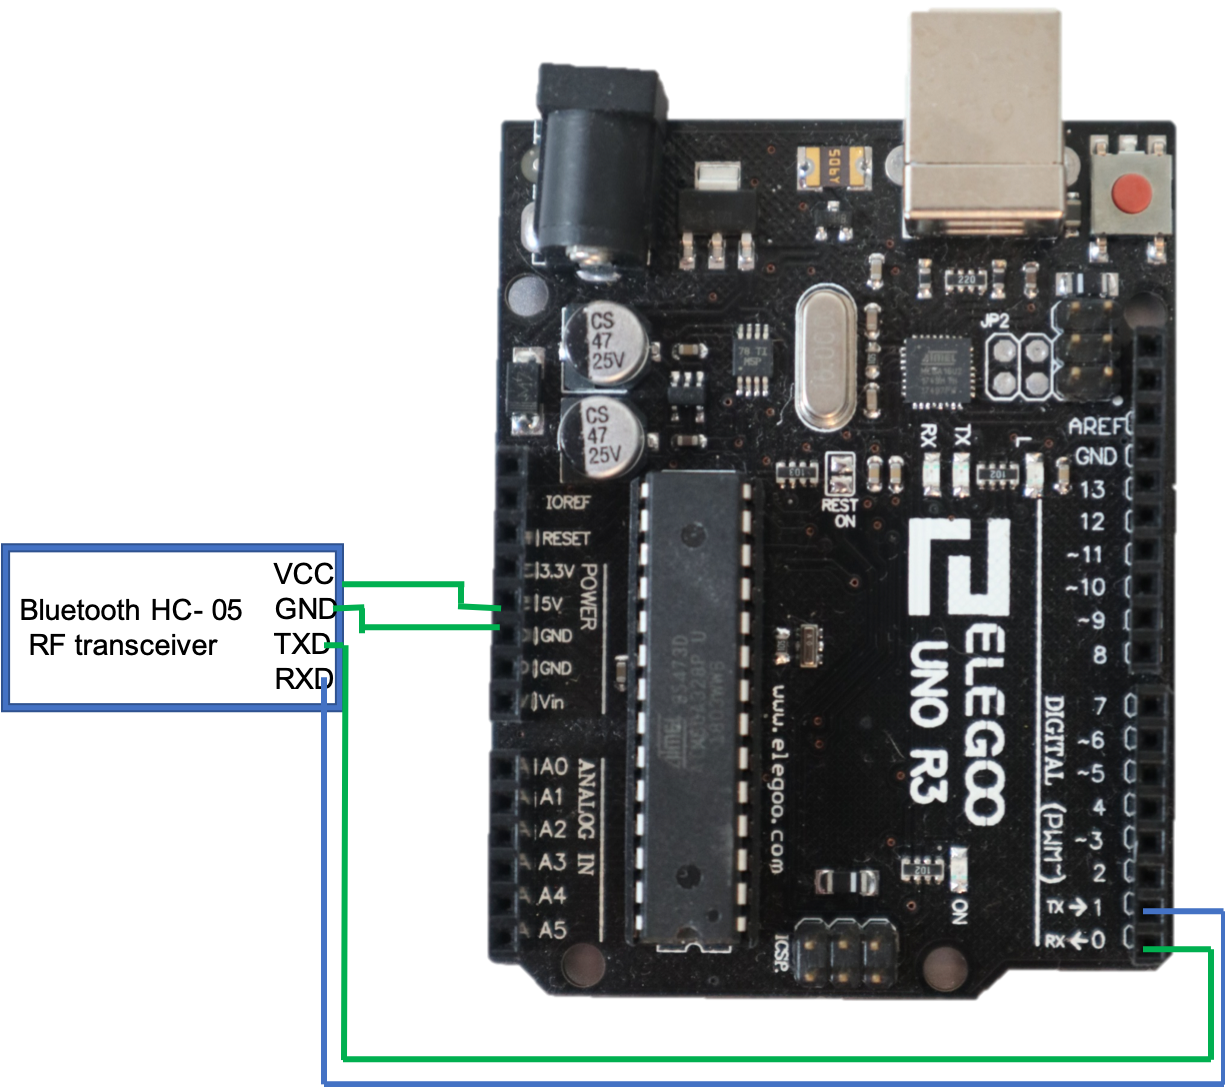
\includegraphics[width=\textwidth, height=100mm]
    {arduino/arduino.png}
    \caption{Arduino layout}
    \label{fig:arduino}
\end{figure}

However, this implementation had several failures; to get more accurate readings, the project would need at least three beacons to demonstrate triangulation wherein three signals are emitted from three angles to get an accurate location. During the testing there was only sufficient means for the procurement of one beacon – this led to an inability to fairly showcase the ideal usage, hindering the projects in this method. 

While it was advised by our domain expert that this Bluetooth solution would be the best policy, it was not practicable given our resources. In view of these drawbacks, the hardware proposal was ceased. The research provided the team with enough of the methods and models to pursue a purely theoretical solution. 

\section{Ethical Audit}
% JT Week 2
% complete
In order to be compliant with GDPR, user locations are recorded during the runtime of the application, and upon termination this data is deleted from memory in order to prevent unauthoried access to the user's location. Users are asked initially to give the Bluetooth, camera, and location permissions to use particular functions.

Since the app uses museum map, and exhibition details, the intellectual property for those will not be under the jurisdiction of the team. Rather, the project members owns the intellectual properties of all technologies that are being created and used in conjunction with third-party information. Since assigning data and storing details to specific users was not implemented in this iteration, in future versions the app will need to prevent attacks such as SQL injections.

\section{Challenges}
% Gabe Week 2
% still needs work
The groups ideas were difficult to manifest due to a lack of technological resources and a much larger, but relevant issue; the infancy of the AR, and accurate indoor navigation market-places.

\subsection{Indoor Navigation \& Augmented Reality}
Currently, the market relies on Bluetooth technology in order to bypass the problem. However, for this application, using Bluetooth has disadvantages that can prove crucial success to the project. First, the group would have to have access to multiple Arduinos in order to propagate the necessary number of Bluetooth RSSI signals to get an accurate position on the user. Without enough Arduinos, the group would be at risk evaluating the signals inaccurately due to the compromising of the signals by metallic surfaces. Another issue with the Bluetooth technology is the risk that it places the user in. 

The group initialised the solution by finding a prototype that had already existed. \note{cite the paper} Once found, another challenge arose; the prototype was last maintained in 2016 so the code did not function to begin with. This hurdle was solved by delegating a sprint to the debugging the application. So a number of Arduinos via Goldsmith College to debug this prototype thoroughly. As the request but the university was deflected and eventually ignored so the only viable option was to purchase Arduinos eventually find that the code would not work without resources that the group had not planned on using. 

This halted the software development of the application for a period of time, until the prevailing solution had been devised. This solution would involve the group hard-coding the geometry of the geospace to be traversed by the user. And using the coded geospace along with a hard-coded location anchor within that geospace to navigate (A-Star algorithm with a vector function as the heuristic) the users device.

Finding problems with AR Core library, the group had problems debugging since documentation was vague and information was scarce. An example of a faced issue was the inability to have the AR section of the application open up on different mobile devices.

\annote{So in retrospect the group could have done a better job with evaluating the history of AR and Indoor Navigation. Because if the group had done so thoroughly to begin with. The group would have been better prepared to tackle problems - avoiding the large halts that arose due to poor resources. However, it proves that the group had an affinity for being adaptively resourceful making it a positive experience in the end.}{not so keen on this point}

\note{might be better to revisit this, until after the back-end implementation is complete}